
To test the CAM logic module a test bench was developed. In this test bench we start by changing the input signal isTranslated to 1 and PC signal to 0x11, in the next clock cycle, when this signal is high the module will check is the PC received is already translated, and as it is not, the output signal notTranslated is set to high state. When this happens, a new tag is added saving the PC and the starting address os the translation.
Then we simulate two check for room instructions. When this happens the output signal oaddr is set with the address in which the processor should store the instruction he wants to store. To obtain this adrress, the module sums the starting address of the basic block, that in this case is 0x0a, with the current basic block size, in this case 0.
To fully test the isTranslated instruction, we simulate another isTranslated instruction, but now as a basic block has already been translated, the notTranslated signal remains low, and the oaddr signal is set with the starting address of the basic block with the saved PC equal to the input PC signal, in this case 0x0a.

\begin{figure} [H]
	\centering
	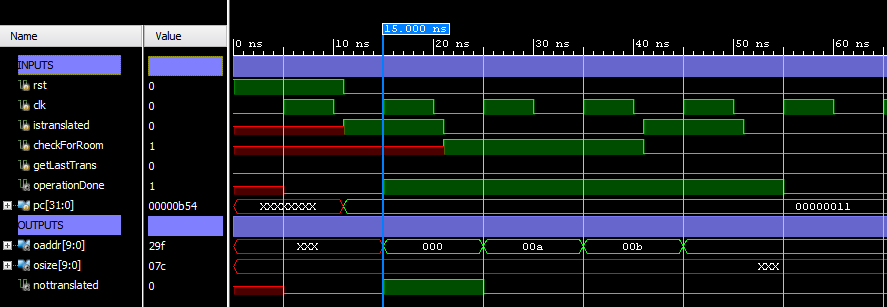
\includegraphics[scale = 0.5]{Images/TestBench1.png}
	\caption{First TestBench: is translated instruction}
	\label{fig:TestBench1}
\end{figure}

In figure \ref{fig:TestBench4} it's possible to see the test to the getLastTrans instruction, at the positive edege of the clock if this signal is high the oaddr will be set to the starting address of the last basic block translated. Firstly we check if the PC 0x11 is translated and, as it is not, a new tag is added automaticaly, then we check for room twice, and then when we set the getLastTrans we can see that the oaddr is set to 0x0a, starting address of the basic block.

\begin{figure} [H]
	\centering
	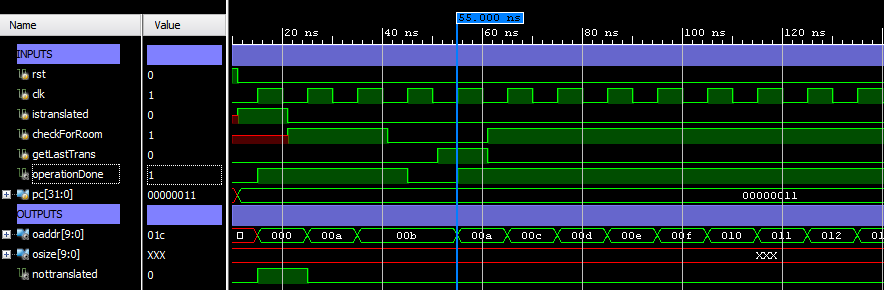
\includegraphics[scale = 0.5]{Images/TestBench4.png}
	\caption{Second TestBench: is translated instruction}
	\label{fig:TestBench4}
\end{figure}

In the figure \ref{fig:TestBench2} we can see that, when we check is the PC 0 is translated, a new tag is added, and the starting address in the translation cache for that basic block is equal to the previous basic block address plus the previous basic block size. We can see that the first address for translation for the new basic block is 0x70 that is equal to the previous basic block address plus the previous basic block size, 0x69, plus 1.

\begin{figure} [H]
	\centering
	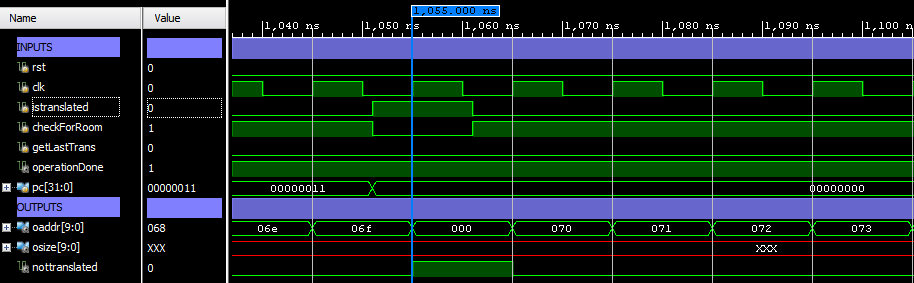
\includegraphics[scale = 0.5]{Images/TestBench2.png}
	\caption{Third TestBench: is translated instruction}
	\label{fig:TestBench2}
\end{figure}

Finally we tested the case where the basic block starting address plus the basic block size surpasses the translation cache size.The cache size is set to 0x400 (1024), and in the following figure, we can see that the basic block starting address is 0x3f4. It's also possible to see that when the basic block size is 13 ( 0x3ff-0x3f4-1) and we try to check if there is room for a new instruction, the oaddr addr is set to the initial address of the basic block,0x3f4, and the osize is set to,0x00c(13), so that, in software the microprocessor can copy the basic block to the starting address of the translation cache. The basic block that was stored there is removed, and the starting address of the basic block is updated to 0x000. When the user checks for room for a new instruction the oaddr is set to 0x00d, the starting address (0x000) plus the basic block size(0x00c) plus 1, that equals 0x00d.

\begin{figure} [H]
	\centering
	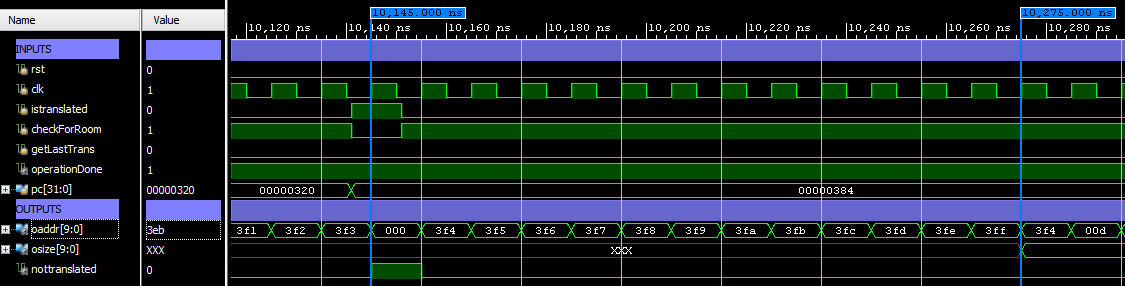
\includegraphics[scale = 0.5]{Images/TestBench3.png}
	\caption{Forth TestBench: is translated instruction}
	\label{fig:TestBench3}
\end{figure}